\section{eo\-Rnd\-Generator$<$ T $>$ Class Template Reference}
\label{classeo_rnd_generator}\index{eoRndGenerator@{eoRndGenerator}}
By popular demand re-introducing a base class for a family of random number generators.  


{\tt \#include $<$eo\-Rnd\-Generators.h$>$}

Inheritance diagram for eo\-Rnd\-Generator$<$ T $>$::\begin{figure}[H]
\begin{center}
\leavevmode
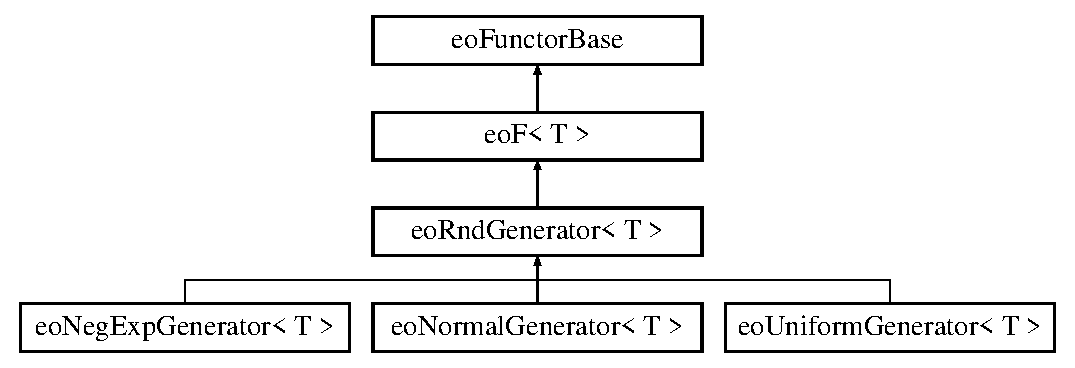
\includegraphics[height=4cm]{classeo_rnd_generator}
\end{center}
\end{figure}
\subsection*{Private Types}
\begin{CompactItemize}
\item 
typedef T {\bf Atom\-Type}\label{classeo_rnd_generator_y0}

\end{CompactItemize}


\subsection{Detailed Description}
\subsubsection*{template$<$class T$>$ class eo\-Rnd\-Generator$<$ T $>$}

By popular demand re-introducing a base class for a family of random number generators. 

Derived members of this class are useful to initialize fixed/variable length genotypes that have an 'atomic' type in an indepent way (thus without employing any knowledge about the problem domain).

See derived classes {\bf eo\-Uniform\-Generator}{\rm (p.\,\pageref{classeo_uniform_generator})}, {\bf eo\-Boolean\-Generator}{\rm (p.\,\pageref{classeo_boolean_generator})}, {\bf eo\-Normal\-Generator}{\rm (p.\,\pageref{classeo_normal_generator})} and {\bf eo\-Neg\-Exp\-Generator}{\rm (p.\,\pageref{classeo_neg_exp_generator})} 



Definition at line 47 of file eo\-Rnd\-Generators.h.

The documentation for this class was generated from the following file:\begin{CompactItemize}
\item 
eo\-Rnd\-Generators.h\end{CompactItemize}
